
\chapter{Soluções para Internet of Things}

Nesta secção será apresentada a \sr que impulsionará toda esta dissertação. Serão descritas as principais características desta planta, principais propriedades e as diferentes aplicações alimentais existentes no mercado. 

	\cite{Our2013}

\section{Evolução tecnologia: o IoT}


Antes de descrever a importância e o conceito de \ac{IoT}, é necessário entender as diferenças entre os termos Internet e \ac{WWW}, que são usados indistintamente pela sociedade. A Internet é a camada ou rede física composta por \textit{switches}, \textit{routers} e outros equipamentos [3]. A sua principal função é transportar informações de um ponto para outro de forma rápida, confiável e segura. Por outro lado, a Web pertence à camada de aplicações que opera sobre a Internet cuja função é oferecer uma interface que transforme as informações que fluem pela Internet em algo útil. Ao longo do tempo, a Web passou e continua a passar por várias etapas evolucionárias, identificadas como:

\begin{itemize}
	\item Web 1.0 – passado: esta primeira etapa foi inventada por Tim Berners Lee em 1989 [5]. Nesta fase surgiram os principais conceitos que conhecemos da Internet atual: Localizador Uniforme de Recursos (do inglês \ac{URL}), Linguagem de Marcação de Hipertexto (do inglês \ac{HTML}) e Protocolo de Transferência de Hipertexto (do inglês \ac{HTTP}). Ainda nesta primeira fase, mas mais tarde, em 1998 foi criado por Larry Page e Sergey Brin o Google que criou simplicidade nas pesquisas na Web [6]. 
	
	\item Web 2.0 – presente: a Web cresceu muito e muito rapidamente. A versão mais próxima da visão de Tim Berners Lee – colaborativa, usado como meio de interação, comunicação global e elevado compartilhamento de informação. 
	
	\item Web 3.0 – futuro: para o futuro prevê-se que os conteúdos online possão vir a estar organizados de forma semântica, muito mais personalizados para cada utilizador, sites, aplicações inteligentes e/ou publicidade baseada nas pesquisas e nos comportamentos.
\end{itemize}

O aparecimento do IoT foi extraordinariamente importante já que se trata da primeira evolução real da Internet, um salto que levará, no futuro, ao desenvolvimento de aplicações revolucionárias com potencial para melhorar significativamente a forma como a sociedade vive, aprende, trabalha e se diverte. O IoT já transformou a Internet em algo sensorial, através da medição de diferentes características, como por exemplo a temperatura, a pressão, as vibrações, a iluminação, a humidade, o stress, entre outras. 


\begin{figure}[!htb]
	\centering
	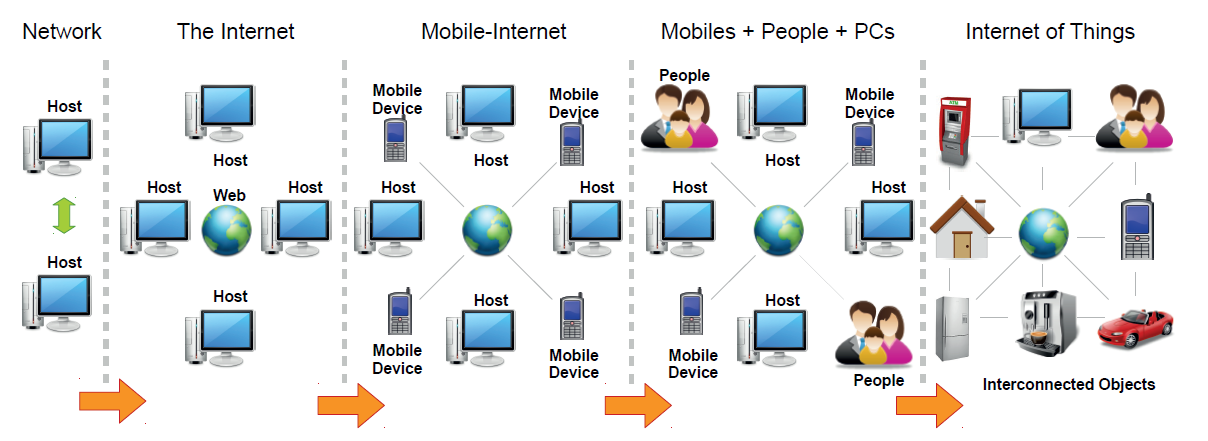
\includegraphics[scale=0.5]{img/cap3-iot/diagrama-evolution.png}
	\caption{Salicornia proveniente da ria de Aveiro}
	\label{Rotulo}
\end{figure}




\section{Tecnologias de comunicação usadas em \ac{IoT}}


\subsection{Bluetooth}

\subsection{WiFi}


\subsection{NFC (Near Field Communication)}

\ac{NFC}


\subsection{Zigbee}



\subsection{Sigfox}

\subsection{LoRa}


\subsection{GSM}



\subsection{Comparação de tecnologias de comunicação}





\ac{IoT}


\section{Aplicações relacionadas}

Seja para comparar, seja para replicar boas funcionalidades, ou seja para conseguir oferecer
algo mais ao utilizador final, quando se pretende desenvolver uma determinada aplicaçao, e
importante proceder a uma avalia¸c˜ao de aplicacoes da mesma area se encontram no mercado.
Assim, s˜ao aqui abordadas algumas das aplica¸c˜oes relacionadas que s˜ao mais utilizadas ou
que mais se aproximam daquilo que se pretende para a aplica¸c˜ao a desenvolver neste projeto,
tendo em conta os diferentes sistemas operativos.

